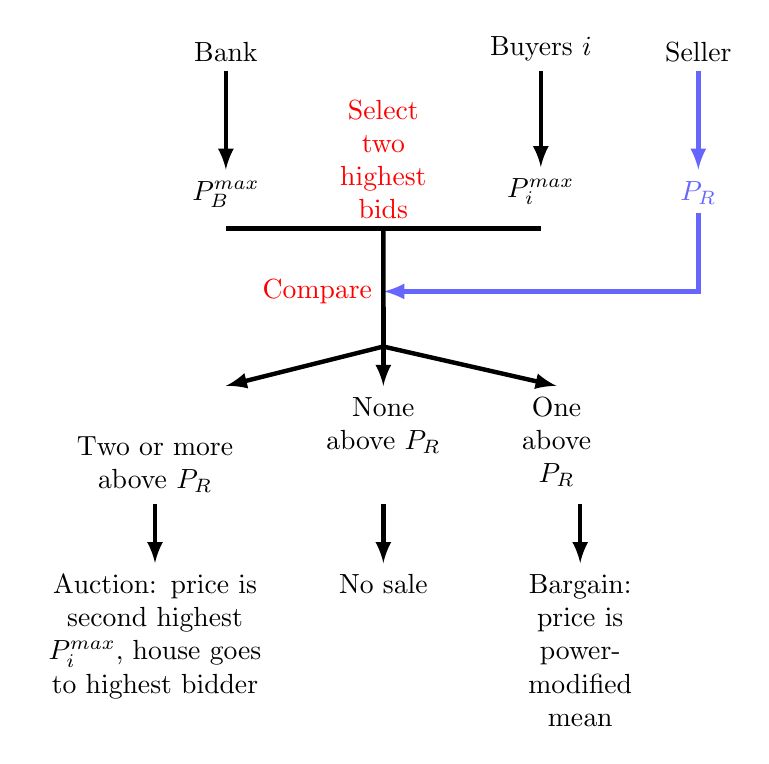
\begin{tikzpicture}
%\draw[step=0.5cm,color=gray] (0,-3) grid (8,7);
\node [above](Bank)at (1,7) {Bank};
\node [above](Buyers)at (5,7) {Buyers $i$};
\node [above](Seller)at (7,7) {Seller};

\draw[ultra thick, -latex](Bank)--++(0,-1.5)node[below]{$P_B^{max}$};
\draw[ultra thick, -latex](Buyers)--++(0,-1.5)node[below]{$P_i^{max}$};
\draw[ultra thick, blue!60,-latex](Seller)--++(0,-1.5)node[below]{$P_R$};

\node[above, red, text width=1.55cm, align=center]at (3,5){Select two highest bids};

\begin{scope}[shift={(0,-1)}]
\draw[ultra thick](1,6.)--(5,6.0); % Bar
\draw[ultra thick, blue!60,-latex](7,6.2)--++(0,-1)--++(-4,0)node[left, red]{Compare};  %Pass P_R to if-then
\draw[ultra thick, -latex](3,6)--++(0,-1.5)--++(-2.,-.5);% down and left
\draw[ultra thick, -latex](3,5)--++(0,-1)node[below, text width=1.5cm, align=center]{None above {$P_R$} };%
\draw[ultra thick, -latex](3,5)--++(0,-.5)--++(2.2,-.5)node[below, text width=1.cm, align=center]{One above {$P_R$} };
% down and Right

\draw[ultra thick, -latex](.1,2.5)node[above, text width=2.cm, align=center]{Two or more above {$P_R$} }--++(0,-.75)node[below, text width=3cm, align=center]{Auction: price is second highest $P_i^{max}$, house goes to highest bidder};

\draw[ultra thick, -latex](3,2.5)--++(0,-.75)node[below, text width=2cm, align=center]{No sale};

\draw[ultra thick, -latex](5.5,2.5)--++(0,-.75)node[below, text width=2cm, align=center]{Bargain: price is power-modified mean};
\end{scope}

\end{tikzpicture}